\subsection{CAM6 aqua-planet simulations}\label{sec:APE}
The 'CESM simpler models' effort also supports aqua-planet configurations \citep{MWO2016JAMES}. The aqua-planet configurations \citep{NH2000ASL} refer to an ocean covered planet with no axial tilt -- a planet in a perpetual equinox and devoid of continents. The aqua-planet compsets designate a fixed, zonally-symmetric SST distribution, modeled after the present day SST distribution on Earth ('QOBS' in \cite{NH2000ASL}). The lack of a seasonal cycle allows one to compute robust statistics from a shorter simulation, and the absence of land removes any influence of discretized topography or interactions with the land model from the simulations. The aqua-planet configurations are therefore an indispensable tool for testing design choices in global atmospheric models.

To understand how the design choices adopted by CAM-SE influence the aqua-planet solutions compared to its predecessor, CAM-HOMME, we ran a pair of simulations using the CAM6 physics package {\color{red}{[CAM6 reference]}} for 4.5 years. Figure~\ref{fig:kespectra} shows the total kinetic energy spectrum at the 200 hPa level in the two simulations. Compared to CAM-HOMME, the slope of the kinetic energy spectrum in CAM-SE is shallower for wavenumbers larger than 30, bringing the solutions closer to the empirically \citep{NG1985JAS} and theoretically \citep{C1971JAS} determined slope of -3 at synoptic scales. The increased kinetic energy at smaller scales is primarily a result of the smaller divergence damping coefficient used in CAM-SE (not shown).

 Figure~\ref{fig:dzonal} shows the zonally averaged total precipitation rate in CAM-HOMME (purple) and CAM-SE (red) averaged over the final 4 years of the simulations. The differences between the two simulations is provided as the purple curve on the bottom plot of Figure~\ref{fig:dzonal}. CAM-SE has increased precipitation at the equator, with a peak difference of 3 mm/day. An approximate 1 mm/day reduction in precipitation occurs on the flanks of the equator (Figure~\ref{fig:dzonal}). CAM-HOMME has twin Inter-Tropical Convergence Zones (ITCZ) straddling the equator, which appears absent from the CAM-SE simulations (Figure~\ref{fig:dzonal}). The total precipitation rate in the model is the sum of the precipitation due to the deep convective parameterization, and that due to CLUBB, which contains shallow convective precipitation and large-scale condensation. The deep convective precipitation rate indicates that the double-ITCZ does exist in CAM-SE (not shown), but is hidden from the total precipitation rate due to the increase in large-scale condensation at the equator.

An analysis of the vertically integrated, zonally averaged dry static energy budget indicates that the latent heating due to the change in precipitation rate are balanced by the anomalous dry static energy flux convergence due to the increase in the mean resolved vertical upward motion at the equator (the dynamic component from eqn. (3) in \cite{MO2011NATUREC}; not shown). This balance also holds for the reduction in precipitation rate on the flanks of the equator (not shown). It is likely that an increase in resolved vertical upward motion in CAM-SE drives the increase in large-scale condensation rate observed in CAM-SE, consistent with a prior analysis of CAM-HOMME \citep{OETAL2016JAMES}. In this scenario, greater downward motion observed on the flanks of the equator are simply compensating for the increased mass flux at the equator, which then acts to stabilize the column and reduce the precipitation rate locally.

The authors have identified three design aspects of CAM-SE that explain the large changes in precipitation observed in the Tropics. These three design aspects are: the use of a lower divergence damping coefficient, a thermodynamically consistent definition of $c_p$ (see \eqref{eq:cp}) and the removal of the limiter in the vertical remapping of the horizontal winds. Figure~\ref{fig:dzonal} shows the total precipitation rate from three additional CAM-SE simulations, each simulation having one of the three modifications reverted back to the CAM-HOMME design. By using the larger divergence damping coefficients from CAM-HOMME in CAM-SE ('CAM-SE-oldvisc'), the precipitation rate at the equator is reduced by about 1 mm/day compared with CAM-SE. The CAM-SE simulation in which the limiter is turned on (CAM-SE-ppmlimiter), as it is in CAM-HOMME, results in a dramatic increase in equatorial precipitation of 3-4 mm/day compared with CAM-SE (Figure~\ref{fig:dzonal}). Through reverting the definition of $c_p$ back to the CAM-HOMME definition ($c_p = c_p^{(d)}$; 'CAM-SE-cpcnst'), the near equatorial precipitation rates are dramatically reduced by 3-4 mm/day (Figure~\ref{fig:dzonal}). A forth simulation was performed containing all three of the aforementioned modifications ('CAM-SE-all'). The simulated total precipitation rates in CAM-SE-all are indistinguishable from the CAM-HOMME simulation (Figure~\ref{fig:dzonal}).
 
The influence of the new definition of $c_p$ and the PPM limiter on Tropical precipitation are not nearly as intuitive as the influence of the divergence damping coefficient. In our aqua-planet simulations, the ITCZ in part, consists of under-resolved, deep convective towers simulated by the resolved dynamics, consistent with a prior study of CAM-HOMME \citep{HR2017JCLIM}. An increase in divergence damping reduces the magnitude of vertical pressure velocities, likely explaining the reduction in precipitation in that simulation. The base of the convective towers often originate within the boundary layer, with convergent flow driving resolved upward mass fluxes through the cloud base. In the CAM-SE-ppmlimiter simulation, the magnitude of the horizontal velocities in the lowest model level of the equatorial convergence zone are larger (Figure~\ref{fig:zonal_v}). The authors speculate that the limiter will select a larger magnitude horizontal wind in the lowest model level in a convergent flow regime, resulting in greater convergence, vertical motion and therefore precipitation. 

To explain how the limiter works, consider a vertical profile of the horizontal wind, $u_k$, in the aqua-planet simulations across the lowest model level, $k$=1, and the second lowest model level, $k$=2 (Figure~\ref{fig:schematic}). In the equatorial regions, there is a monotonic increase in the magnitude of the wind with height, across the lowest three levels. If level 1 is undergoing horizontal mass convergence, the model level will be raised (Figure~\ref{fig:schematic}). To find the lowest model level wind on the new grid, $u_{\tilde 1}$, one integrates the PPM subgrid reconstruction from the surface to within a region that is occupied by level $k$=2. If the limiter is on, it forces the contribution of the wind to $u_{\tilde 1}$ from the $k$=2 layer to be equal to $u_2$. Since the magnitude of the wind increases with height, the contribution of the wind in $u_{\tilde 1}$ from the region occupied by level $k$=2 will always have a smaller magnitude than $u_2$, which is computed by integrating to the top of the $k$=2 layer, where the winds are largest (Figure~\ref{fig:schematic}). In this scenario, the limiter will result in larger magnitude winds in the lowest model level, facilitating greater mass convergence during the following time-step.    

The influence of a thermodynamically consistent definition of $c_p$ is to increase precipitation near the equator by 3-4 mm/day (Figure~\ref{fig:dzonal}). Note that the $c_p=c_p^{(d)}$ change affects not only the energy conversion term in the thermodynamic equation but also the frictional heating term and the vertical remapping of temperature. Additional aqua-planet simulations reveal two important reasons for this sensitivity. A simulation in which $c_p = c_p^{(d)}$ only in the frictional heating term (equation \eqref{eq:tcp}), results in a reduction in equatorial precipitation of 1-2 mm/day (not shown). This result is intuitive, since the term $\left(\vec{v}\cdot \delta \vec{v}\right)$ is always negative, the heating rate is inversely proportional to $c_p$. In CAM-SE, $c_p$ is always greater than $c_p^{(d)}$, and so there is more frictional heating in CAM-SE than there is in CAM-HOMME. In the equatorial regions, additional heating likely facilitates buoyancy, which increases resolved vertical motion, leading to an increase in precipitation. Setting $c_p = c_p^{(d)}$ just in the energy-conversion term in the thermodynamic equation also leads to a reduction in precipitation rates. We speculate that this is due to the reduced forcing term in the $T$-equation (third term on left-hand side of \eqref{E:PEtemp}) that in turn leads to larger densities (reduced temperature leads to increased density through the ideal gas law all else being equal) that then reduce the pressure gradient force (fourth term on left-hand side of \eqref{E:PEmom}) and therefore less convergence in the Equatorial `belt' of precipitation.

\begin{figure}[h]
\centering
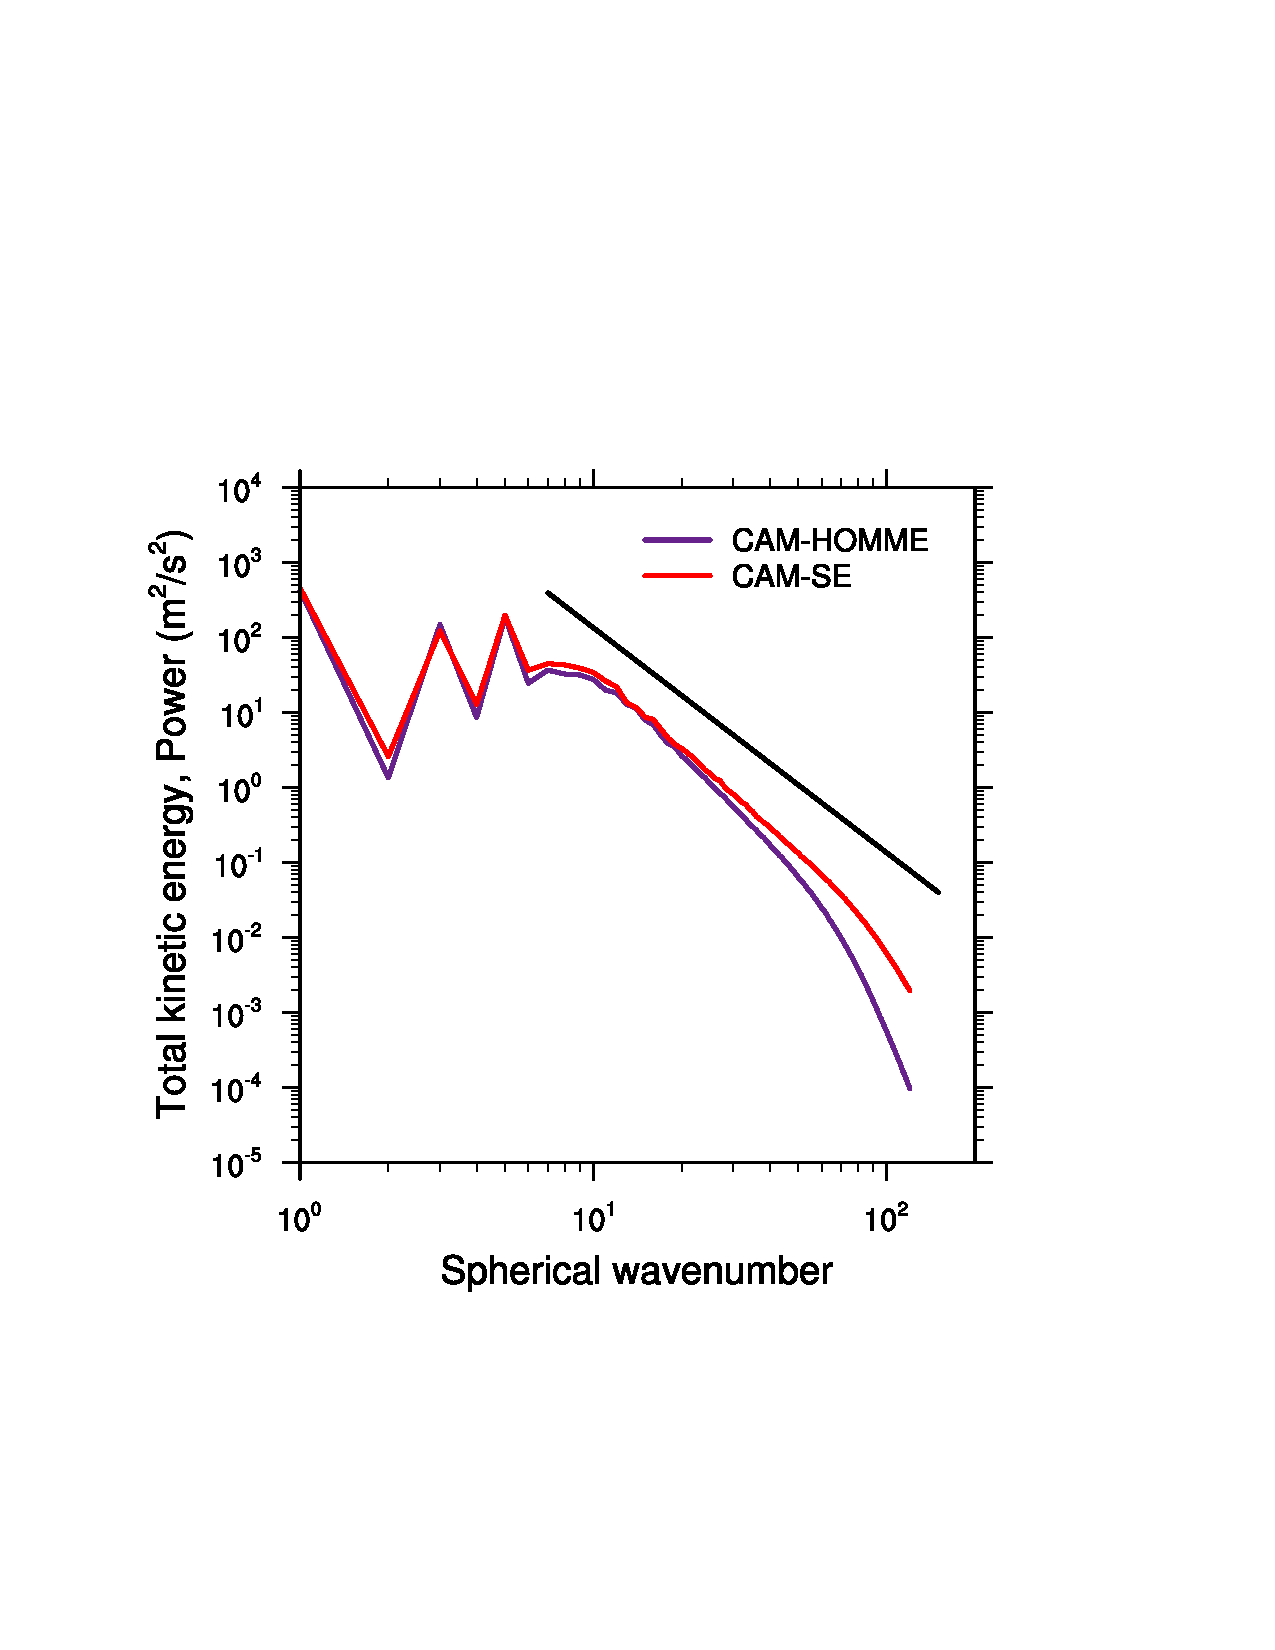
\includegraphics[width=20pc]{figs/kespectra.pdf}
\caption{Total kinetic energy spectrum of the horizontal winds at the 200 hPa level in CAM-HOMME and CAM-SE, computed as the mean spectra 30 days of 6-hourly instantaneous spectra. Black line is the $k^{-3}$ reference scaling.}
\label{fig:kespectra}
\end{figure}

\begin{figure}[h]
\centering
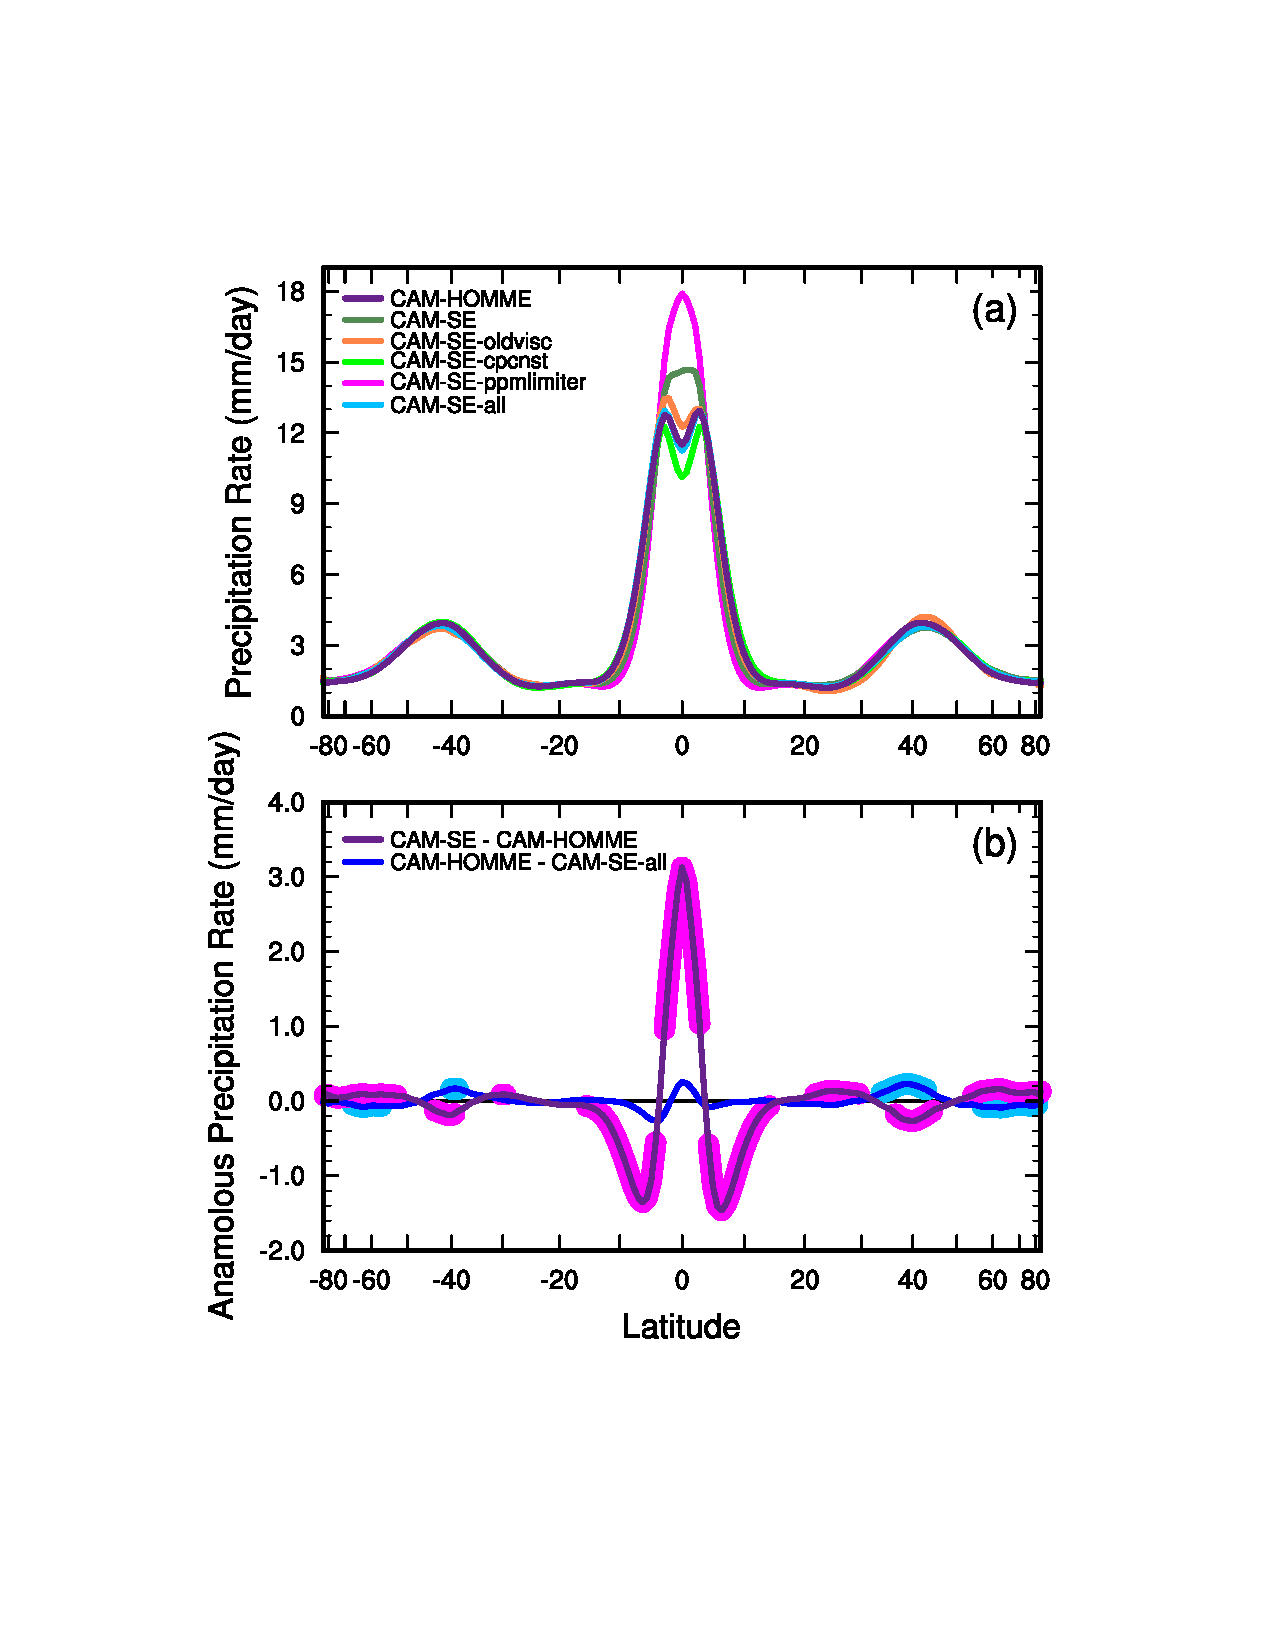
\includegraphics[width=20pc]{figs/dzonal_prect.pdf}
\caption{(Upper) The zonally average total precipitation rates in the aqua-planet simulations, averaged over the final 4 years of a 4.5 years simulation. Labels are defined in the text (lower) The change in the total precipitation rate between two simulations denoted by the label. The shading indicates where the differences are significant at the 95\% confidence level.}
\label{fig:dzonal}
\end{figure}

\begin{figure}[h]
\centering
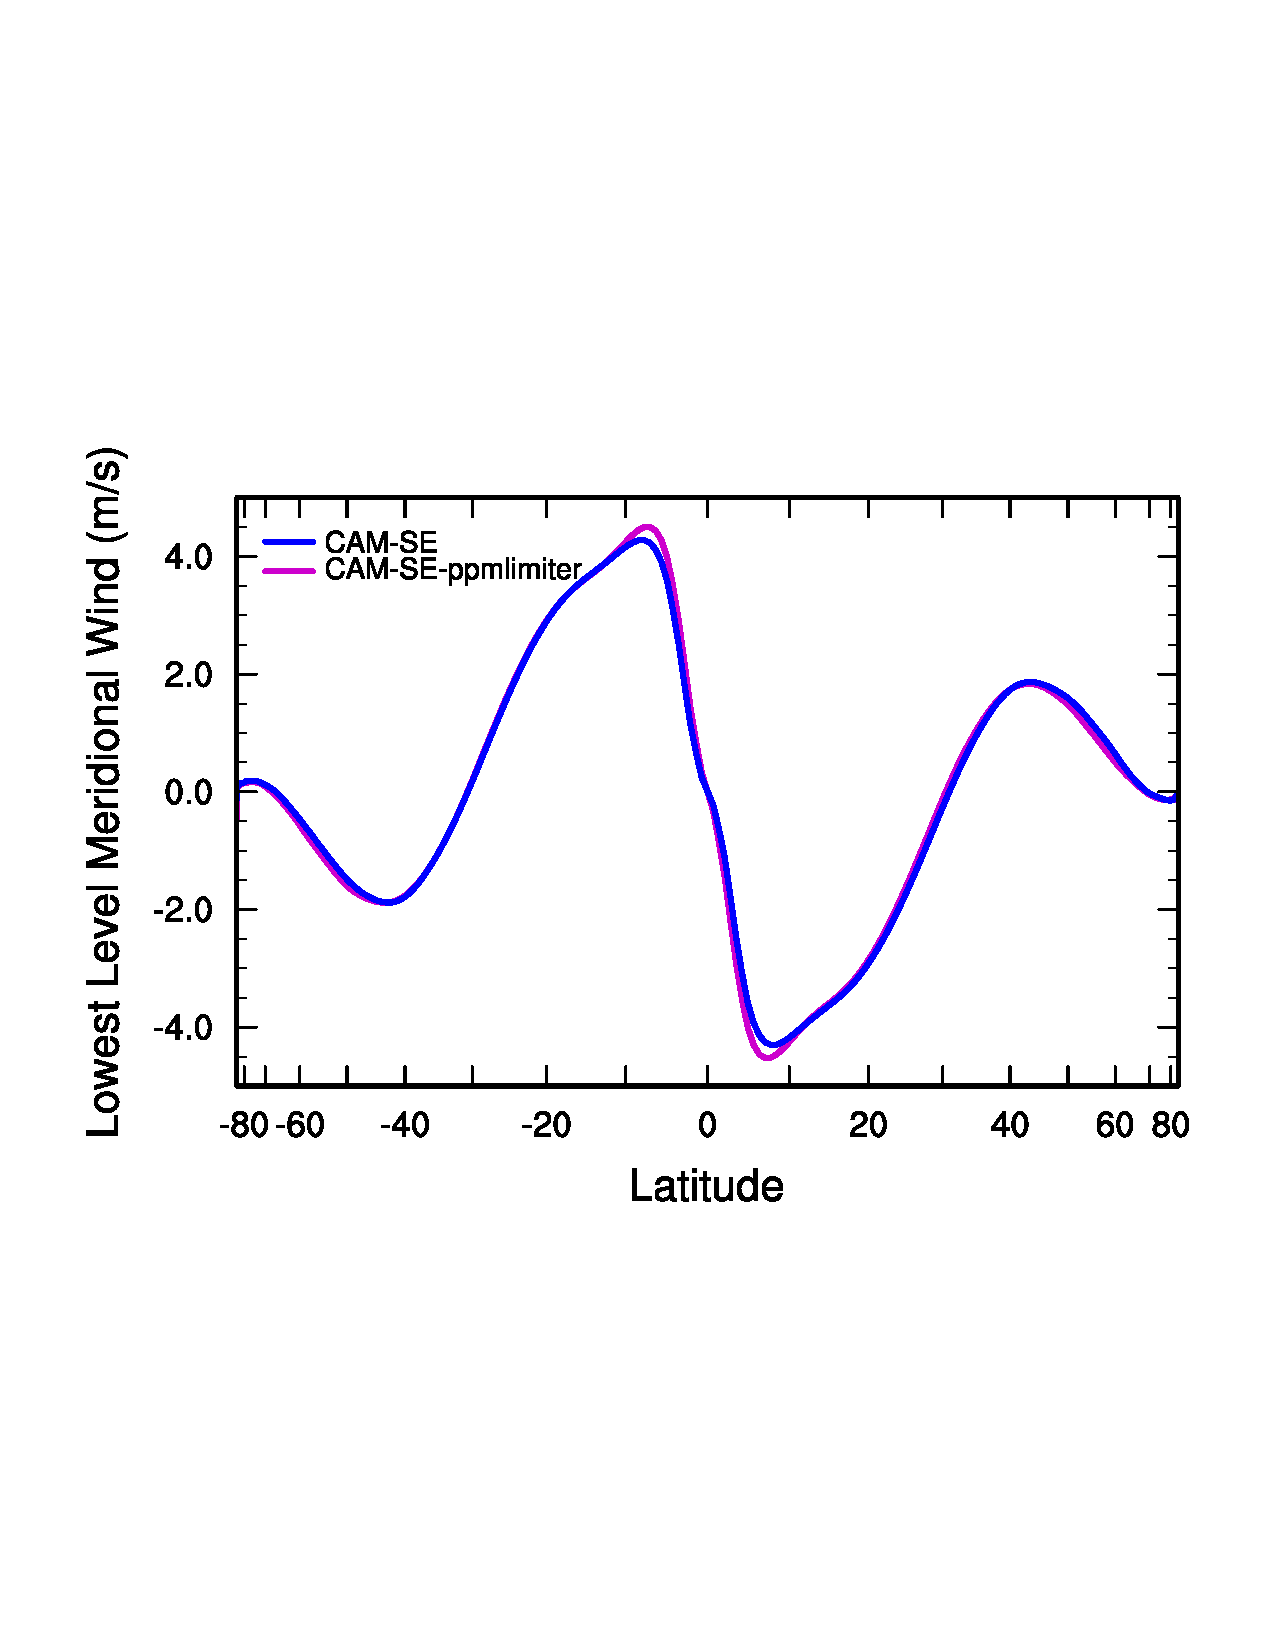
\includegraphics[width=20pc]{figs/zonal_v.pdf}
\caption{Time-mean, zonally averaged lowest model level meridional wind in the CAM-SE and CAM-SE-ppmlimiter simulations, computed from the entirety of a 4.5 year simulation.}
\label{fig:zonal_v}
\end{figure}

\begin{figure}[h]
\centering
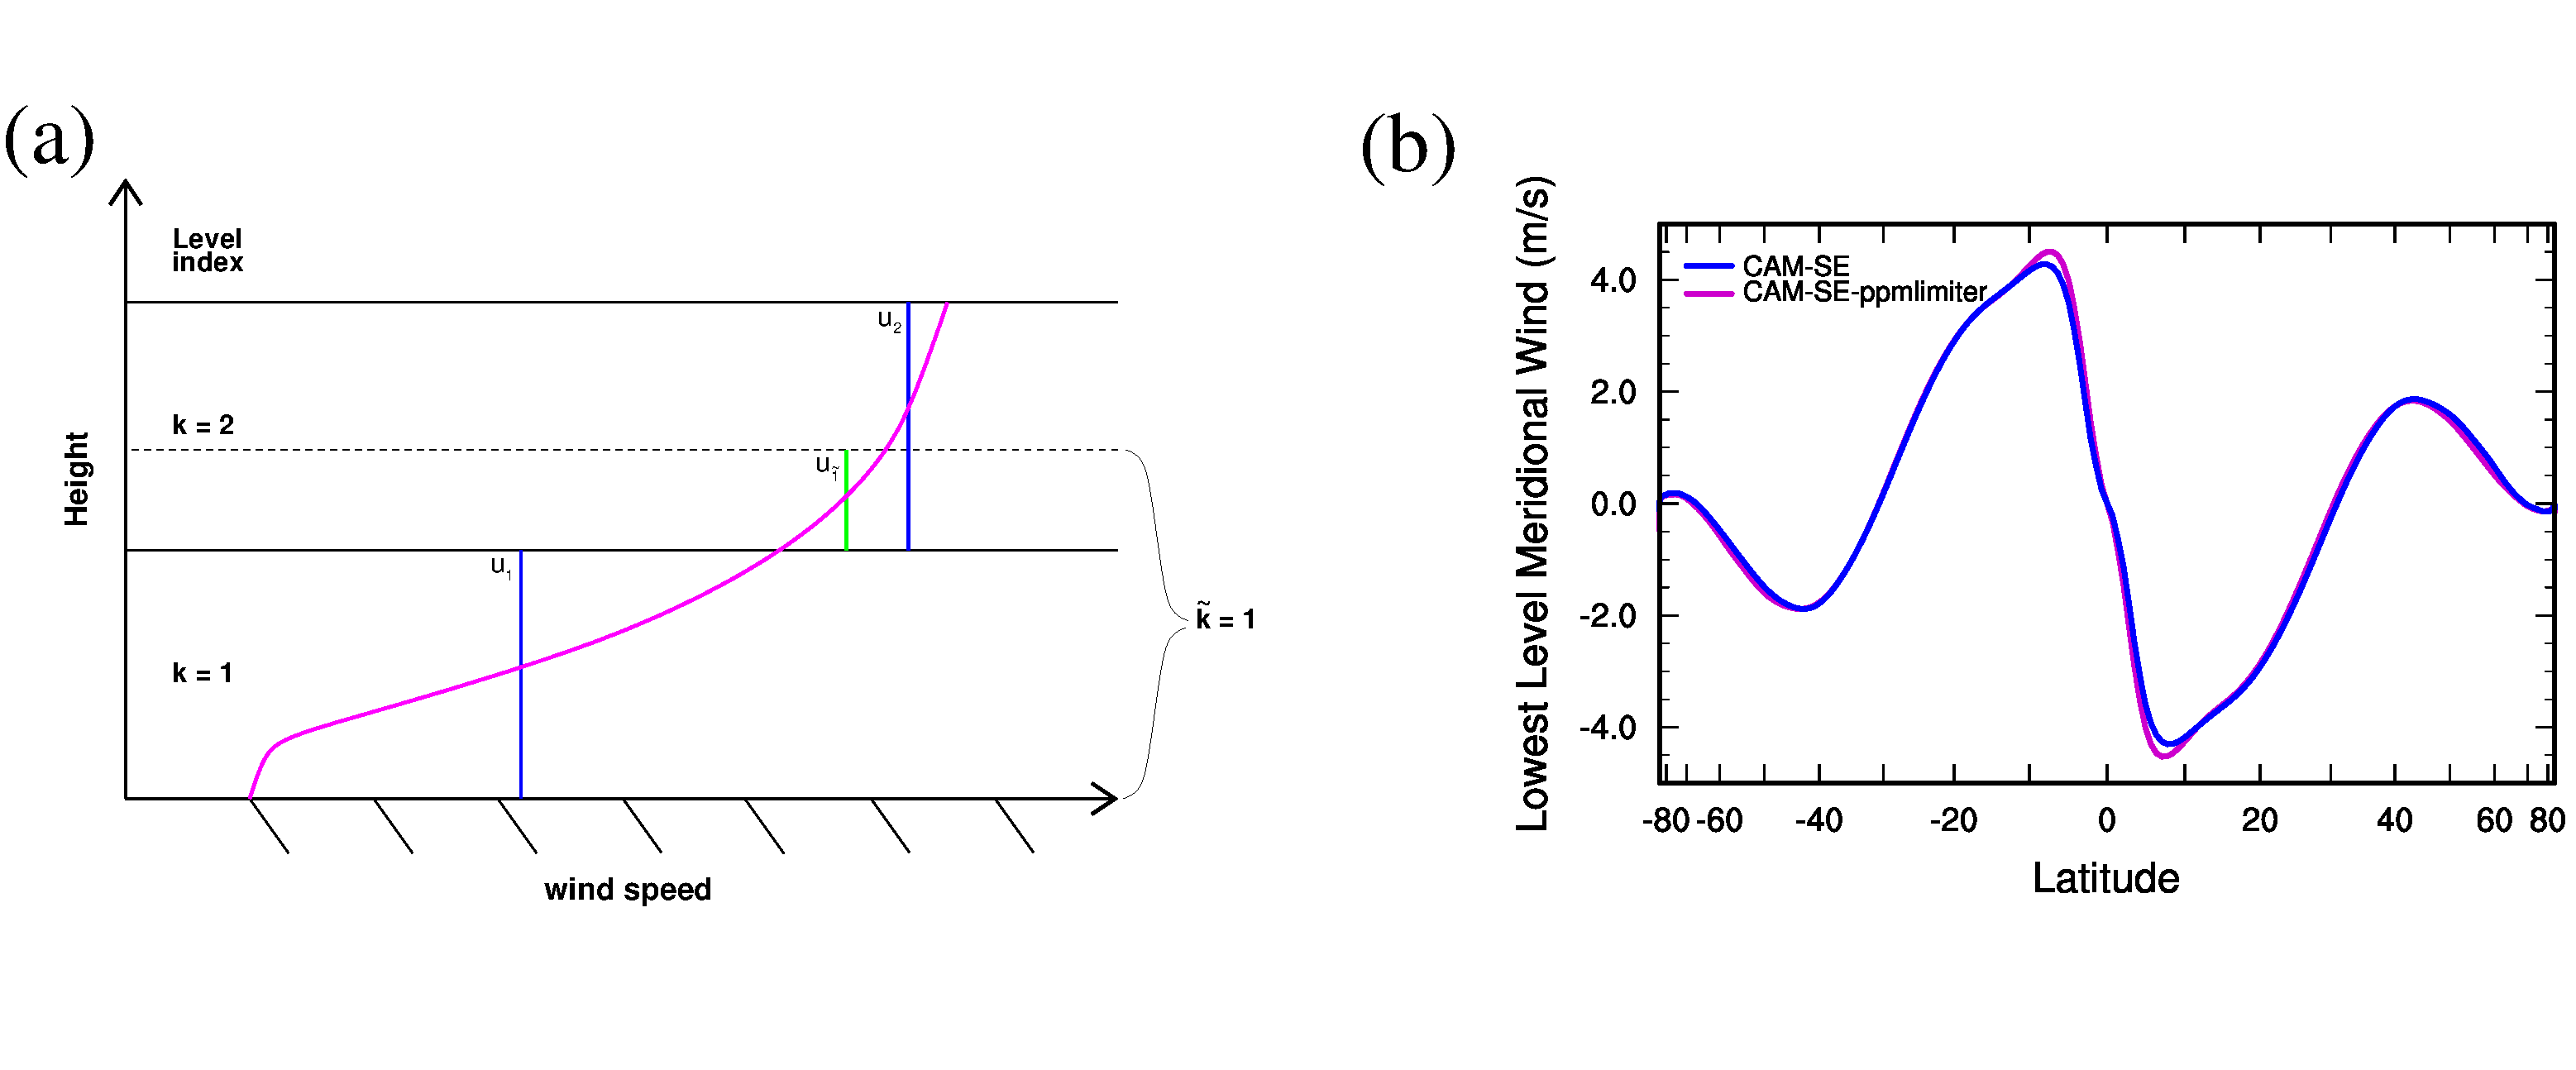
\includegraphics[width=20pc]{figs/schematic.pdf}
\caption{A schematic illustration of the influence of the limiter on the vertical remapping of the winds of the lowest model level, in a convergent flow regime. Solid black lines show the layer interface, and the dashed line shows the top of the lowest model level in the following time-step. The model winds are denoted as blue-bars, while the PPM reconstruction is shown as the pink curve. The green bar is the wind computed by integrating the reconstruction from the top of level 1 to the top of level 1 in the following time-step. Notations are provided in the text.}
\label{fig:schematic}
\end{figure}

